% PGF/TikZ notes
% Produce vector graphics from geometric/algebraic descriptions
\documentclass{article}
\usepackage{graphicx} % demonstration and helps for self annotating

\usepackage{tikz}
% \usetikzlibrary{} - load additional libraries
% e.g. "arrows", "automata", "mindmap", "petri", etc.

\begin{document}

% simple right angles
\begin{figure}
\centering{}
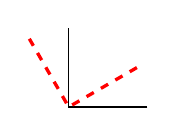
\begin{tikzpicture}
\draw (1,0) -- (0,0) -- (0,1);
\draw[red, dashed, very thick, rotate=30] (1,0) -- (0,0) -- (0,1);
\end{tikzpicture}
\caption{Right angle}
\end{figure}

% simple right triangle
\begin{figure}
\centering{}
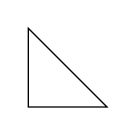
\begin{tikzpicture}
\draw (1,0) -- (0,0) -- (0,1) -- cycle;
\end{tikzpicture}
\caption{Right triangle}
\end{figure}

\end{document}